\documentclass{jomas}

\addbibresource{jomas.bib}

% JoMAS Article Metadata
\arttitle{Electronic Service Quality and Customer Complaint Handling on Food Delivery Platforms: An Empirical Service Operations Study of Nasi Gerilya on GrabFood}
\artauthors{Marsia Br Pelawi$^{1*}$, Tetty Yuliaty$^2$, Arlina Nurbaity Lubis$^2$, Haryaji Catur Putera Hasman$^2$}
\artaffiliations{$^1$Undergraduate in Management, Faculty of Economics and Business, Universitas Sumatera Utara, Medan, Indonesia\\$^2$Department of Management, Faculty of Economics and Business, Universitas Sumatera Utara, Medan, Indonesia}
\artemail{$^*$marsiabr@students.usu.ac.id}

\begin{document}

\makejomasheader

\begin{abstract}
Online food delivery platforms require small restaurants to manage service quality and customer satisfaction effectively. This study analyzes electronic service quality, order fulfillment bottlenecks, and complaint management at Nasi Gerilya Restaurant on GrabFood in Medan City. We examine 4,584 GrabFood customer reviews, observe kitchen queue operations, and interview nine key informants across management, kitchen staff, cashiers, IT consultants, consumers, and competing restaurants. The restaurant maintains strong customer satisfaction through consistent food taste, generous meat portions, and responsive dish replacements. However, peak lunch hours create operational bottlenecks because dine-in customers, takeaway buyers, and delivery couriers crowd a single service counter. Packaging omissions, wrong food variants, and soup spillage cause recurring customer complaints. We map the order fulfillment process through a service blueprint and identify five operational failure points across e-service quality dimensions. We recommend a two-stage fail-safe packaging checklist, a separate courier dispatch station, and tamper-evident packaging to eliminate fulfillment errors and protect customer retention.
\end{abstract}
\keywords{e-service quality, complaint handling, GrabFood, service operations, service blueprint.}

\section{INTRODUCTION}
Online food delivery has become a primary commercial channel for urban restaurants in post-pandemic Indonesia \parencite{elverda2025ofdindonesia}. Urban consumers choose food delivery apps for convenience and fast doorstep delivery \parencite{chaffey2022digitalmarketing}. For food and beverage small enterprises, platform partnerships expand customer reach without expanding physical dining space \parencite{kotler2023principlesmarketing}. Food delivery platforms connect culinary merchants to large consumer bases through algorithmic matching and integrated payment gateways \parencite{pigatto2017fooddelivery}.

However, digital merchants face unique operational challenges. On delivery platforms, customers evaluate service quality through app responsiveness and order accuracy rather than dining room hospitality \parencite{parasuraman2005esqual,zeithaml2002service}. Four core dimensions define this electronic service quality: fulfillment accuracy, system efficiency, menu availability, and dispute resolution \parencite{parasuraman2005esqual}. Unlike dine-in restaurants where staff can resolve mistakes tableside, fulfillment errors on digital platforms immediately damage customer ratings \parencite{santoso2023esatisfaction}. These operational defects include omitted condiments, swapped food items, and extended driver waiting times. Public customer reviews display these failures directly to prospective buyers.

Nasi Gerilya is a Padang restaurant in Medan City operating since September 2024. The restaurant generates approximately 50\% of its daily transactions from GrabFood. Nasi Gerilya maintains a strong online reputation with an average rating of 4.7 out of 5.0 across 4,584 reviews. The restaurant also achieved GrabFood \textit{Rising Star} awards in 2025 and 2026. However, high transaction volumes cause severe congestion during lunch hours between 11:30 and 13:30 WIB. A single frontline counter processes dine-in orders, walk-in takeaway sales, and online driver pickups. Customer reviews reflect recurring complaints regarding missing condiments, swapped dishes, and driver waiting delays.

Existing literature predominantly examines consumer adoption drivers of food delivery applications \parencite{putri2022grabfood}. Few empirical studies investigate operational fulfillment bottlenecks inside restaurant kitchens. This study examines e-service quality dimensions at Nasi Gerilya on GrabFood. We identify specific failure points during order preparation and propose an operational service recovery framework.

\section{LITERATURE REVIEW}
\textcite{parasuraman2005esqual} developed the e-service quality framework to evaluate online transactions across four core dimensions: efficiency, fulfillment, system availability, and privacy. Efficiency measures user interface speed and ease of navigation. Fulfillment covers delivery timeliness and order accuracy. System availability describes catalog accuracy and technical uptime. Privacy protects customer personal data. On food delivery platforms, fulfillment accuracy represents the most visible dimension to end consumers \parencite{santoso2023esatisfaction}.

In food services, order fulfillment connects the digital order to the physical food delivery \parencite{wirtz2024servicesmarketing}. The service marketing 7P mix emphasizes processes, people, and physical evidence \parencite{kotler2023principlesmarketing}. Physical evidence includes menu photos, item descriptions, receipt labels, and tamper-evident packaging. When delivered food does not match the app listing, customers experience a service failure. Quick staff responses, item replacements, and apologies restore customer trust \parencite{wirtz2024servicesmarketing,smith1999servicerecovery}. In contrast, slow or defensive merchant responses reduce customer return rates.

Physical service environments also shape customer and employee behavior. \textcite{bitner1992servicescapes} established the servicescape framework to explain how spatial layout, equipment placement, and ambient conditions affect operational flow. In multi-channel restaurants, physical counter crowding creates direct friction between walk-in patrons and delivery couriers. To prevent service errors during peak transaction velocity, service operations require mistake-proofing mechanisms. \textcite{chase1994failsafe} formulated fail-safe service design (poka-yoke) to eliminate human errors during order preparation. In food packaging, structured checklists ensure complete meal assembly before dispatch.

\section{METHODS}
This study applies a descriptive qualitative single-case design \parencite{yin2018casestudy}. We investigate order fulfillment operations at Nasi Gerilya Restaurant in Medan City. The single-case approach provides deep empirical access to kitchen processes, physical counter workflows, and digital review telemetry.

\subsection{Sampling and Informant Profile}
We selected nine key informants through purposive sampling across management, kitchen operations, frontline cashiers, IT consultants, active platform consumers, and competing restaurants. Informants possess direct knowledge of GrabFood store operations, meal packaging, and multi-channel queuing. Table~\ref{tab:informant-profile} displays the informant matrix and operational competencies.

\begin{table}[H]
\caption{Key Informant Matrix and Operational Competencies}
\label{tab:informant-profile}
\centering
\small
\begin{tabularx}{\textwidth}{c l l X}
\toprule
\textbf{No.} & \textbf{Informant} & \textbf{Role / Position} & \textbf{Operational Competency and Scope} \\
\midrule
1 & Richard & Business Owner & Strategic channel mix, quality control, and POS software \\
2 & Ririn & Frontline Leader \& Cashier & GrabFood POS, queue management, and order mediation \\
3 & Bella & Kitchen Assembler & Meal assembly, ingredient portioning, and box packing \\
4 & Devin & Business Consultant (APINDO) & Store layout advisory, queue flow, and process audits \\
5 & Alip & Active Consumer & Order accuracy, meal completeness, and missing gravy issues \\
6 & Reyza & Active Consumer & Promotion transparency, meat portions, and delivery speed \\
7 & Ojan & Active Consumer & Student meal bundles, value perception, and food taste \\
8 & Ken & Staff, RM Pondok Krakatau & Competitor packaging, driver queues, and stockout delays \\
9 & Asiong & Staff, RM Istana Krakatau & Competitor dispatch routines and dine-in vs delivery flows \\
\bottomrule
\end{tabularx}
\end{table}

\subsection{Data Collection}
We collected empirical data through four distinct methods:
\begin{enumerate}[leftmargin=*,itemsep=1pt,topsep=1pt]
    \item \textbf{Digital Content Analysis}: We examined 4,584 GrabFood customer reviews from June 13, 2026.
    \item \textbf{In-Depth Interviews}: We interviewed nine informants using semi-structured protocols covering order preparation, packaging checks, driver handovers, and complaint resolution.
    \item \textbf{Direct Observation}: We observed receipt printing, meal assembly, packaging, and courier handovers during peak lunch hours (11:30--13:30 WIB).
    \item \textbf{Document Audits}: We audited GrabFood menu structures, pricing records, 19 promotional voucher terms, and stockout registers.
\end{enumerate}

\subsection{Data Analysis}
We analyzed qualitative data using the interactive model of \textcite{miles2014qualitative}. This model includes data condensation, matrix displays, and conclusion drawing. We compared interview transcripts with platform data and observational notes.

\section{RESULTS}
Fieldwork reveals that Nasi Gerilya maintains high customer satisfaction on GrabFood. However, operational bottlenecks slow down order preparation and dispatch.

\subsection{Digital Storefront Audit and Platform Performance}
Table~\ref{tab:storefront-parameters} outlines the audited storefront parameters. The storefront displays an aggregate rating of 4.7 out of 5.0 from 4,584 reviews and GrabFood \textit{Rising Star} badges. However, several popular items remain out of stock on the app.

\begin{table}[H]
\caption{Operational Storefront Parameters Audited on GrabFood}
\label{tab:storefront-parameters}
\centering
\small
\begin{tabularx}{\textwidth}{c l X}
\toprule
\textbf{No.} & \textbf{Storefront Parameter} & \textbf{Empirical Observation Findings (June 13, 2026)} \\
\midrule
1 & Outlet Identity \& Rating & Nasi Gerilya - Glugur Kota; Rating 4.7 / 5.0 (4,584 verified customer reviews) \\
2 & Recognition Badges & GrabFood \textit{Rising Star} Winner 2025 \& 2026 (5-Star Restaurant Designation) \\
3 & Promotional Campaigns & 19 active promotional vouchers (bank, discounts, delivery subsidies) \\
4 & Signature Dishes & Beef Rendang, Spiced Fried Chicken Rice, and Creamy Pop Chicken Rice \\
5 & Price Range & Rp1,100 (additional curry sauce) to Rp72,000 (premium multi-dish packages) \\
6 & Catalog Stockouts & 6 items marked \textit{Sold Out} (premium fish head and packaged sambals) \\
\bottomrule
\end{tabularx}
\end{table}

When customers order dishes that the kitchen has run out of, staff must call buyers to change menus or cancel orders.

\begin{figure}[t]
\centering
\begin{subfigure}[b]{0.48\textwidth}
    \centering
    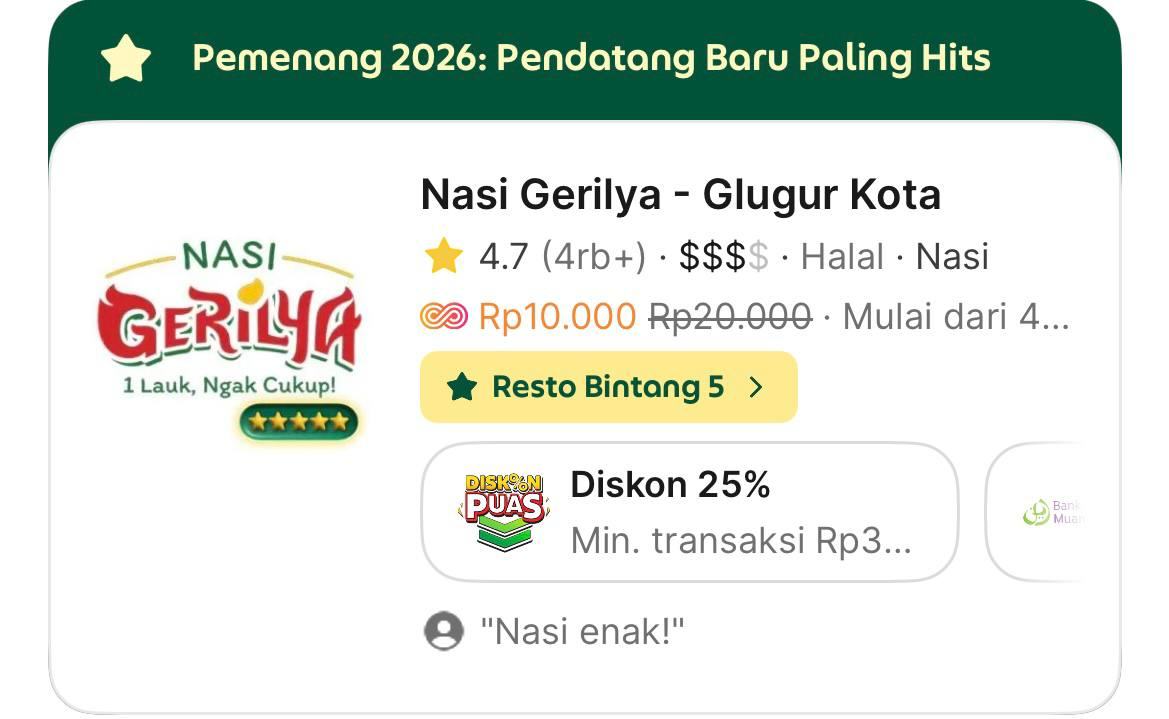
\includegraphics[width=\textwidth,height=4.2cm,keepaspectratio]{../resource/05-fieldwork/02-observasi-grabfood/user-supplied/nasi-gerilya-grabfood-profil-pemenang-2026.jpg}
    \caption{Digital Storefront and Rating Badges}
    \label{fig:storefront}
\end{subfigure}
\hfill
\begin{subfigure}[b]{0.48\textwidth}
    \centering
    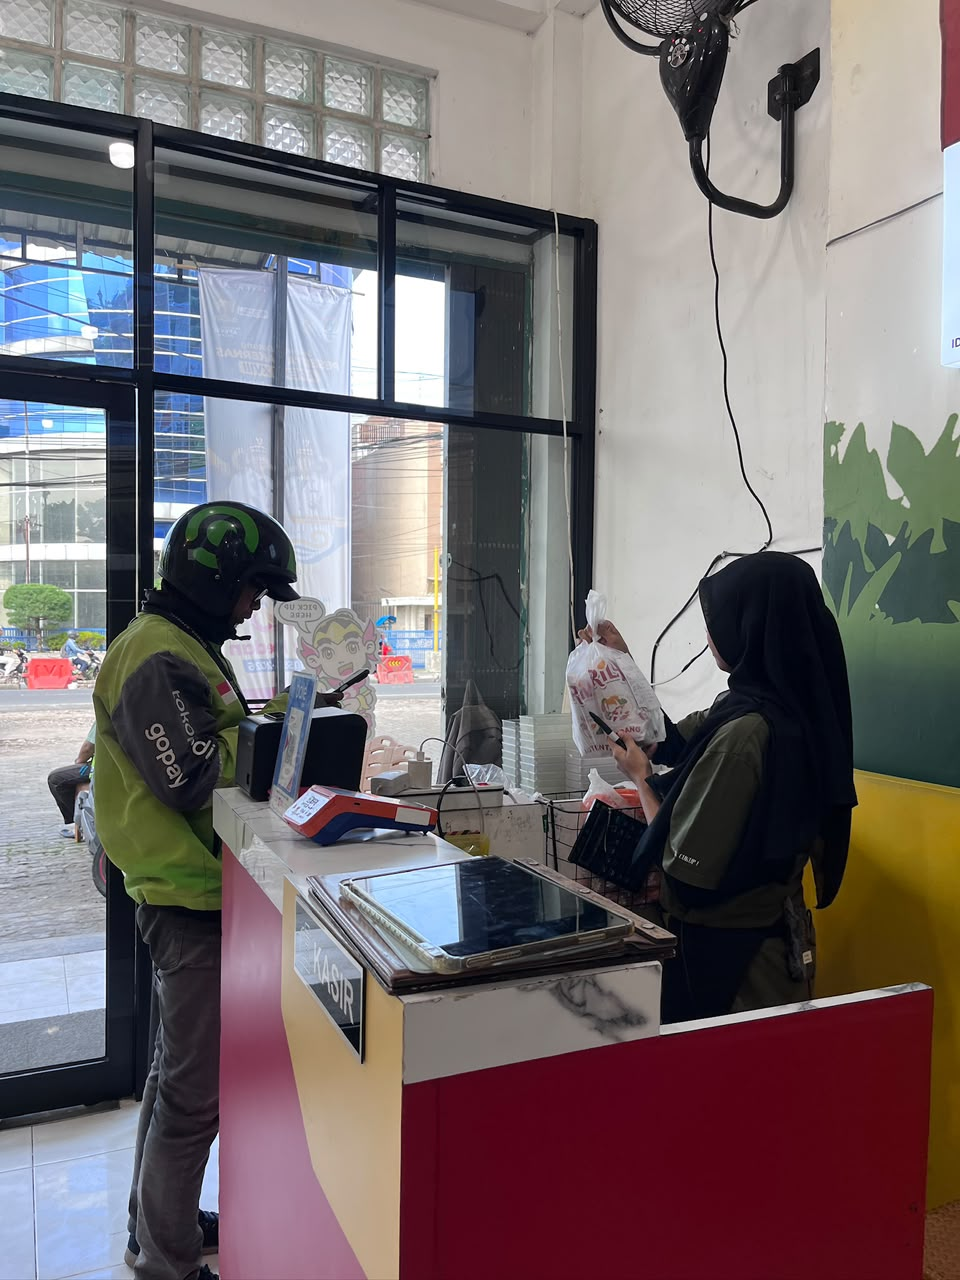
\includegraphics[width=\textwidth,height=4.2cm,keepaspectratio]{../resource/05-fieldwork/01-wawancara/20260701-20260704-wawancara-lapangan/kasirgerilya.jpg}
    \caption{Frontline Cashier Workstation}
    \label{fig:cashier}
\end{subfigure}
\caption{Digital Interface and Physical Fulfillment Workstation at Nasi Gerilya}
\label{fig:storefront-and-cashier}
\end{figure}

Figure~\ref{fig:storefront-and-cashier} displays the digital storefront alongside the physical cashier counter. Figure~\ref{fig:cashier} shows a single counter handling dine-in guests, takeaway buyers, and delivery drivers. This layout creates severe congestion during peak hours.

To examine catalog availability friction, Table~\ref{tab:soldout-inventory} lists the six menu items marked unavailable during platform observation.

\begin{table}[H]
\caption{Audit of Unavailable Menu Items on GrabFood Storefront}
\label{tab:soldout-inventory}
\centering
\small
\setlength{\tabcolsep}{5pt}
\begin{tabularx}{\textwidth}{c p{5.6cm} c X}
\toprule
\textbf{No.} & \textbf{Menu Item Name} & \textbf{Price (Rp)} & \textbf{Operational Stockout Category} \\
\midrule
1 & Gulai Merah Kepala Ikan (Size L) & 275,000 & Premium fish item; limited daily procurement \\
2 & Gulai Merah Kepala Ikan (Size M) & 248,050 & Premium fish item; limited daily procurement \\
3 & Nasi Padang Gembung Kuring Bakar & 47,850 & Fresh fish dish; exhausted before lunch peak \\
4 & Nasi Padang Ayam Pop Creamy & 46,000 & Core signature dish; high customer demand \\
5 & Sambal Cumi Nagih Kemasan & 38,500 & Packaged retail item; batch production run delay \\
6 & Sambal Tuna Asap Keumamah Aceh & 38,500 & Packaged retail item; batch production run delay \\
\bottomrule
\end{tabularx}
\end{table}

Table~\ref{tab:soldout-inventory} demonstrates that stockouts affect both high-ticket specialty seafood and best-selling core dishes. Unsynchronized inventory causes immediate customer disappointment when users attempt to reorder signature items.

\subsection{Promotional Architecture and Inventory Friction}
Table~\ref{tab:promo-schemes} details the 19 active promotional vouchers on GrabFood. Commercial bank partnerships dominate promotions and attract new buyers. However, the restaurant does not sync kitchen inventory with the POS terminal. As a result, the digital menu displays exhausted dishes.

\begin{table}[H]
\caption{Distribution of Active Promotional Campaigns and Inventory Stockouts}
\label{tab:promo-schemes}
\centering
\small
\begin{tabularx}{\textwidth}{c l c X}
\toprule
\textbf{No.} & \textbf{Promotional Mechanism} & \textbf{Items} & \textbf{Operational Terms and Merchant Objective} \\
\midrule
1 & Commercial Bank Co-Marketing & 11 & Minimum spend Rp40k--Rp100k; discounts Rp4k--Rp25k \\
2 & Merchant-Funded Percentage Off & 2 & 17\%--25\% discount (capped at Rp50k--Rp100k) \\
3 & Delivery Subsidization & 3 & Rp3,000--Rp8,000 discount; offsets customer delivery cost \\
4 & Dish-Level Deduction & 1 & Direct Rp4,500 price reduction applied to Minced Meat Curry \\
5 & Collaborative Group Order & 1 & 5\% discount for 3--6 joint orders \\
6 & Stockout Friction Points & 6 & Snapper Head Curry and sambal jars \textit{Sold Out} \\
\bottomrule
\end{tabularx}
\end{table}

Bank promotions attract budget-conscious buyers and drive lunch order surges. These surges quickly deplete popular dishes in the kitchen. The cashiers must then call customers manually to negotiate meal replacements.

\subsection{Menu Architecture and Pricing Tier Distribution}
Table~\ref{tab:menu-pricing} presents menu categories and price distributions. Menu tiers range from vegetable rice at Rp27,500 to mutton curry at Rp72,000. À la carte proteins cost between Rp27,000 and Rp67,500.

\begin{table}[H]
\caption{Menu Architecture and Pricing Tiers on GrabFood Storefront}
\label{tab:menu-pricing}
\centering
\small
\begin{tabularx}{\textwidth}{c l c c X}
\toprule
\textbf{No.} & \textbf{Menu Category} & \textbf{Count} & \textbf{Price Range (Rp)} & \textbf{Representative Core Items} \\
\midrule
1 & Complete Rice Packages & 26 & 27,500 -- 72,000 & Rendang Sapi, Ayam Pop, Kari Kambing \\
2 & Additional Side Dishes & 7 & 7,700 -- 27,500 & Jengkol Rendang, Telur Dadar, Keripik Kentang \\
3 & À La Carte Proteins & 23 & 27,000 -- 67,500 & Gulai Cincang, Ayam Bakar, Udang Goreng \\
4 & Fresh Table Sambals & 2 & 17,500 & Sambal Hijau Lado Mudo, Sambal Merah \\
5 & Bottled Specialty Sambals & 6 & 38,500 & Sambal Andaliman, Cumi Nagih, Teri Medan \\
6 & Gravy Supplements & 2 & 1,100 -- 2,500 & Kuah Gulai Kuning, Kuah Campur \\
\bottomrule
\end{tabularx}
\end{table}

Table~\ref{tab:menu-pricing} shows that complete rice packages dominate the catalog with 26 SKUs. Each box includes rice, meat, vegetables, green chili, and curry gravy. Packing many separate items increases the risk of omitting condiments during lunch rush.

\subsection{Platform Mark-Up and Customer Expectation Asymmetry}
To evaluate the economic factors driving consumer grievance intensity, Table~\ref{tab:price-markup} compares in-store dine-in prices with GrabFood digital prices across core signature dishes.

\begin{table}[H]
\caption{Comparative Pricing Audit: Dine-In vs. GrabFood Platform Mark-Up}
\label{tab:price-markup}
\centering
\small
\setlength{\tabcolsep}{5pt}
\begin{tabularx}{\textwidth}{c l c c c X}
\toprule
\textbf{No.} & \textbf{Core Menu Item} & \textbf{Dine-In (Rp)} & \textbf{GrabFood (Rp)} & \textbf{Mark-Up} & \textbf{Operational Cost Driver and Packaging Allocation} \\
\midrule
1 & Nasi Sayur Polos & 22,000 & 27,500 & +25.0\% & Platform fee (20\%) and partitioned meal box \\
2 & Nasi Ayam Goreng Bumbu & 36,000 & 45,000 & +25.0\% & Platform fee (20\%) and greaseproof box packaging \\
3 & Nasi Ayam Pop Creamy & 37,000 & 46,000 & +24.3\% & Platform fee (20\%) and separate sauce cup \\
4 & Nasi Rendang Sapi & 45,000 & 56,000 & +24.4\% & Platform fee (20\%) and separate gravy cup \\
5 & Nasi Kikil Tunjang Gulai & 55,000 & 68,000 & +23.6\% & Platform fee (20\%) and double-lined takeout tub \\
6 & Nasi Kari Kambing & 58,000 & 72,000 & +24.1\% & Platform fee (20\%) and reinforced soup bowl \\
\bottomrule
\end{tabularx}
\end{table}

Table~\ref{tab:price-markup} demonstrates a consistent 23\%--25\% pricing mark-up on GrabFood across all core packages. This mark-up covers the standard 20\% merchant platform commission and dedicated takeout packaging materials. Field interviews reveal that paying a substantial price premium heightens consumer quality expectations. When online consumers pay Rp56,000 for beef rendang that costs Rp45,000 in-store, an omitted condiment pouch is perceived not as a minor oversight, but as an unacceptable fulfillment failure justifying an immediate 1-star penalty.

\subsection{Service Blueprint and Operational Failure Points}
To analyze how order fulfillment breaks down during peak velocity, we mapped the operational workflow into a service blueprint. Figure~\ref{fig:service-blueprint} illustrates the four physical fulfillment stages and their corresponding failure points.

\begin{figure}[t]
\centering
\begin{tikzpicture}[
    node distance=0.8cm and 0.5cm,
    font=\small,
    box/.style={rectangle, draw=black, thick, fill=gray!10, text width=3.4cm, minimum height=1.3cm, align=center},
    fail/.style={rectangle, draw=black, thick, fill=black!15, text width=3.4cm, minimum height=1.1cm, align=center, font=\footnotesize\bfseries},
    arrow/.style={-{Stealth[scale=1.2]}, thick}
]
\node[box] (step1) {1. Digital Order\\(GrabFood Ingestion)};
\node[box, right=of step1] (step2) {2. Kitchen Assembly\\(Meal Packaging)};
\node[box, right=of step2] (step3) {3. Frontline Dispatch\\(Ticket Verification)};
\node[box, right=of step3] (step4) {4. Courier Transit\\(Last-Mile Delivery)};

\node[fail, below=0.6cm of step1] (fail1) {Failure Point 1:\\Catalog Stockout (6\%)};
\node[fail, below=0.6cm of step2] (fail2) {Failure Point 2:\\Missing Condiments (38\%)};
\node[fail, below=0.6cm of step3] (fail3) {Failure Point 3:\\Dish Swap (18\%)};
\node[fail, below=0.6cm of step4] (fail4) {Failure Point 4:\\Driver Delays (26\%)\\Packaging Spills (12\%)};

\draw[arrow] (step1) -- (step2);
\draw[arrow] (step2) -- (step3);
\draw[arrow] (step3) -- (step4);

\draw[dashed, thick] (step1) -- (fail1);
\draw[dashed, thick] (step2) -- (fail2);
\draw[dashed, thick] (step3) -- (fail3);
\draw[dashed, thick] (step4) -- (fail4);
\end{tikzpicture}
\caption{Service Blueprint of Order Fulfillment Journey and Operational Failure Points}
\label{fig:service-blueprint}
\end{figure}

Figure~\ref{fig:service-blueprint} shows that operational errors concentrate at specific handover boundaries. The kitchen assembly stage generates condiment omissions, while the cashier dispatch stage causes variant mix-ups due to visually identical paper receipts.

\subsection{Empirical Analysis of Customer Grievances}
We coded 4,584 reviews and identified five recurring operational failures. Table~\ref{tab:complaint-categories} explains the root causes observed during restaurant service encounters.

\begin{table}[H]
\caption{Classification of Operational Service Failures Across E-S-QUAL Dimensions}
\label{tab:complaint-categories}
\centering
\small
\setlength{\tabcolsep}{5pt}
\begin{tabularx}{\textwidth}{c l l c X}
\toprule
\textbf{No.} & \textbf{Failure Category} & \textbf{E-S-QUAL Dimension} & \textbf{Share} & \textbf{Root Cause and Mechanism Observed in Fieldwork} \\
\midrule
1 & Missing Condiments & Fulfillment & 38\% & Curry gravy, sambal pouches, or cutlery omitted during lunch rush \\
2 & Driver Waiting Delays & Efficiency & 26\% & Couriers wait 15--25 minutes as staff prioritize in-store patrons \\
3 & Incorrect Menu Variant & Fulfillment & 18\% & Swapped meal boxes caused by visually similar 4-digit order tickets \\
4 & Packaging Spillage & Physical Evidence & 12\% & Loosely fastened gravy pouches tear inside carrier bags in transit \\
5 & Real-Time Stockout & Availability & 6\% & Depleted items remain active digitally, forcing phone cancellations \\
\bottomrule
\end{tabularx}
\end{table}

Fieldwork observations in Table~\ref{tab:complaint-categories} confirm that errors do not come from cooking mistakes. Instead, counter crowding and the absence of a packing checklist cause these failures.

\begin{figure}[b]
\centering
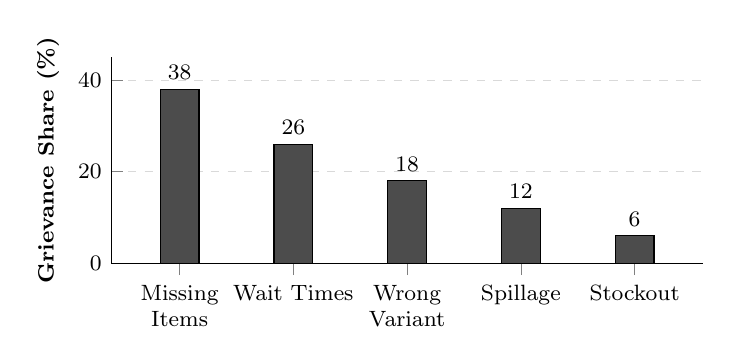
\begin{tikzpicture}
\begin{axis}[
    ybar,
    bar width=14pt,
    width=0.75\textwidth,
    height=4.2cm,
    ymin=0,
    ymax=45,
    ylabel={Grievance Share (\%)},
    symbolic x coords={Missing Items,Wait Times,Wrong Variant,Spillage,Stockout},
    xtick=data,
    nodes near coords,
    nodes near coords align={vertical},
    every node near coord/.append style={font=\footnotesize\bfseries},
    x tick label style={font=\footnotesize, text width=1.6cm, align=center},
    y tick label style={font=\footnotesize},
    ylabel style={font=\footnotesize\bfseries},
    axis lines*=left,
    enlarge x limits=0.15,
    ymajorgrids=true,
    grid style={dashed,gray!30}
]
\addplot[fill=black!70, draw=black] coordinates {
    (Missing Items,38)
    (Wait Times,26)
    (Wrong Variant,18)
    (Spillage,12)
    (Stockout,6)
};
\end{axis}
\end{tikzpicture}
\caption{Quantitative Distribution of Customer Grievance Categories}
\label{fig:complaint-distribution}
\end{figure}

As shown in Figure~\ref{fig:complaint-distribution}, missing items (38\%) and driver waiting times (26\%) account for 64\% of all customer complaints. These two operational issues stem directly from queue bottlenecks and single-checker packing.

\subsection{Triangulated Qualitative Evidence: Staff and Management Insights}
To understand the underlying causes of packaging omissions and queue congestion, we conducted in-depth interviews with internal restaurant personnel. Table~\ref{tab:staff-interview-quotes} compiles representative interview statements from management, kitchen staff, cashiers, and IT consultants.

\begin{table}[H]
\caption{Thematic Coding of Operational Fieldwork Interviews}
\label{tab:staff-interview-quotes}
\centering
\small
\begin{tabularx}{\textwidth}{c l l X}
\toprule
\textbf{No.} & \textbf{Informant} & \textbf{Operational Area} & \textbf{Verbatim Fieldwork Interview Insight} \\
\midrule
1 & Richard & Quality Control & \textit{"Consistency in taste is non-negotiable. If spices fail our standard, we discard the batch. But delivery packing requires stricter oversight."} \\
2 & Bella & Kitchen Assembly & \textit{"During peak rush, packing gets frantic. Items packed in separate plastic pouches, like curry gravy and sambal, are vulnerable to omission."} \\
3 & Ririn & Cashier \& Dispatch & \textit{"Four-digit order codes on printed tickets often look identical. If a driver mentions the wrong code, meal boxes can get swapped."} \\
4 & Devin & Queue Architecture & \textit{"Dine-in, takeaway, and delivery couriers crowd one counter. Without physical lane separation, driver waiting times increase rapidly."} \\
\bottomrule
\end{tabularx}
\end{table}

Table~\ref{tab:staff-interview-quotes} confirms that internal staff recognize the operational friction points. The kitchen leader identifies separate gravy pouches as the primary omission risk, while the cashier attributes dish swaps to visually indistinguishable POS receipts.

\subsection{Representative Digital Review Evidence}
Customer reviews show a sharp contrast between delicious food and fulfillment errors. Table~\ref{tab:review-evidence} presents verbatim customer reviews from the GrabFood storefront.

\begin{table}[H]
\caption{Representative Verbatim Customer Reviews from GrabFood Storefront}
\label{tab:review-evidence}
\centering
\small
\begin{tabularx}{\textwidth}{c l c c X}
\toprule
\textbf{No.} & \textbf{Reviewer ID} & \textbf{Rating} & \textbf{Valence} & \textbf{Verbatim Review Extract and Operational Context} \\
\midrule
1 & Raymond & 5/5 & Positive & \textit{"The pop chicken is creamy, tender, and seasoned to perfection."} \\
2 & Wie W. & 5/5 & Positive & \textit{"Weekly family order; generous portions, clean boxes, requests met."} \\
3 & Talia & 1/5 & Negative & \textit{"Ordered chicken rendang, but received fried chicken instead."} \\
4 & Hendra & 3/5 & Neutral & \textit{"Ordered fish but received tilapia; merchant issued formal apology."} \\
5 & Siyaga & 3/5 & Neutral & \textit{"Food is delicious, but staff omitted extra curry; responsive merchant."} \\
6 & Albert P. & 1/5 & Negative & \textit{"Staff omitted crispy skin crackers; merchant apologized for oversight."} \\
\bottomrule
\end{tabularx}
\end{table}

Table~\ref{tab:review-evidence} shows that consistent taste earns 5-star ratings. However, missing gravy or wrong dishes immediately trigger 1-star ratings. These operational errors undermine customer retention.

\subsection{Cross-Merchant Triangulation: Industry-Wide Fulfillment Dynamics}
To assess whether fulfillment errors represent an idiosyncratic problem of Nasi Gerilya or an industry-wide challenge, we interviewed operational staff from two competing Padang restaurants on GrabFood. Table~\ref{tab:competitor-comparison} compares operational practices across merchants.

\begin{table}[H]
\caption{Comparative Triangulation Across Competing Padang Restaurants on GrabFood}
\label{tab:competitor-comparison}
\centering
\small
\setlength{\tabcolsep}{5pt}
\begin{tabularx}{\textwidth}{c l c p{5.5cm} X}
\toprule
\textbf{No.} & \textbf{Establishment} & \textbf{Online Share} & \textbf{Primary Service Bottlenecks} & \textbf{Fulfillment Recovery Practice} \\
\midrule
1 & Nasi Gerilya & $\sim$50\% & Missing gravy (38\%) and driver wait (26\%) & Instant replacement with merchant apology \\
2 & RM Pondok Krakatau & $\sim$50\% & Driver delays and unsynced stockouts & Missing item redelivery via courier \\
3 & RM Istana Krakatau & $\sim$20\% & Omitted side dishes and lunch rush & Direct manual checker inspection \\
\bottomrule
\end{tabularx}
\end{table}

Table~\ref{tab:competitor-comparison} demonstrates that multi-channel queue crowding and condiment omissions affect competing food merchants across Medan. Therefore, packaging errors and courier wait times represent systemic operational challenges in online food delivery.

\section{DISCUSSION}
These empirical findings substantiate the core propositions of \textcite{parasuraman2005esqual} and \textcite{wirtz2024servicesmarketing}. On on-demand delivery platforms, fulfillment accuracy represents a foundational hygiene factor rather than a secondary differentiator. Customers consistently praise culinary attributes, such as portion volume and authentic Padang seasoning, with 5-star ratings. However, fulfillment failures directly penalize these ratings. When staff omit curry sauce or send the wrong dish, customers immediately assign 1-star reviews. This asymmetric penalty demonstrates that culinary satisfaction cannot compensate for fulfillment errors in digital environments \parencite{santoso2023esatisfaction}.

Furthermore, queue dynamics reveal operational decoupling challenges between physical and virtual service encounters \parencite{bitner1992servicescapes}. The shared frontline counter creates direct interference between dine-in guests and delivery couriers. Cooks prioritize visible seated customers over digital tickets. This queue bias increases driver waiting times and causes courier friction.

To address these vulnerabilities, we structure three operational improvements:

\subsection{Two-Stage Fail-Safe Packaging Protocol}
Packaging errors stem from relying on a single cook during lunch rush hours. The restaurant should implement a two-stage fail-safe checklist \parencite{chase1994failsafe}, structured as an operational poka-yoke inspection routine. Table~\ref{tab:poka-yoke-checklist} outlines the procedural stages, control parameters, and physical mechanisms.

\begin{table}[H]
\caption{Proposed Two-Stage Fail-Safe Quality Verification Checklist}
\label{tab:poka-yoke-checklist}
\centering
\small
\setlength{\tabcolsep}{4.5pt}
\begin{tabularx}{\textwidth}{c l l X l}
\toprule
\textbf{Stage} & \textbf{Inspector} & \textbf{Control Parameter} & \textbf{Inspection Criterion} & \textbf{Poka-Yoke Mechanism} \\
\midrule
1 & Kitchen Packer & Meal Completeness & Rice portion, main protein, and side vegetables & Physical ticket item check \\
1 & Kitchen Packer & Condiments \& Sauces & Curry gravy pouch, sambal pouch, and chili cup & Count of liquid pouches \\
1 & Kitchen Packer & Eating Utensils & Spoon, fork, and hygiene tissue paper & Dedicated cutlery slot fill \\
2 & Frontline Cashier & Ticket Matching & 4-digit GrabFood code vs. driver app display & Verbal and visual code match \\
2 & Frontline Cashier & Transit Security & Heat-resistant lid, taped gravy, and tamper seal & Tamper-evident seal adhesion \\
\bottomrule
\end{tabularx}
\end{table}

Under this protocol, Stage 1 guarantees meal integrity inside the kitchen, while Stage 2 prevents dispatching mismatched order bags to drivers.

\subsection{Servicescape Decoupling and Dedicated Courier Dispatch Station}
Driver waiting times (26\%) occur because delivery couriers and dine-in patrons compete for frontline space. Physical counter crowding degrades service encounters for both groups \parencite{bitner1992servicescapes}. To resolve this spatial friction, Figure~\ref{fig:servicescape-decoupling} contrasts the existing counter layout with the proposed decoupled servicescape model.

\begin{figure}[t]
\centering
\begin{tikzpicture}[
    font=\small,
    thick,
    wall/.style={line width=1.4pt, draw=black!80, fill=gray!2, rounded corners=4pt},
    kitchen/.style={draw=black!60, fill=white, rounded corners=2pt, align=center},
    counter/.style={draw=black!80, fill=black!12, rounded corners=2pt, align=center, font=\bfseries\scriptsize},
    hatch/.style={draw=black!90, fill=black!25, rounded corners=2pt, align=center, font=\bfseries\scriptsize},
    bottleneck/.style={draw=black!70, fill=white, rounded corners=2pt, align=center, font=\bfseries\scriptsize},
    actor/.style={draw=black!60, fill=white, rounded corners=2pt, align=center, font=\scriptsize},
    flow/.style={-{Stealth[scale=0.9]}, line width=1.1pt, draw=black!85},
    driverflow/.style={-{Stealth[scale=0.9]}, line width=1.1pt, dashed, draw=black!85}
]

% =========================================================================
% (a) AS-IS: CONGESTED LAYOUT (SINGLE COUNTER)
% =========================================================================
\node[font=\bfseries] at (3.3, 6.2) {(a) Existing Layout: Shared Single Counter};

% Outer Wall: 6.6cm wide, 5.6cm tall
\draw[wall] (0, 0) rectangle (6.6, 5.6);

% Kitchen BOH
\node[kitchen, text width=6.0cm, minimum height=1.1cm] (k1) at (3.3, 4.65) {
    \textbf{\footnotesize BACK-OF-HOUSE (KITCHEN)}\\[2pt]
    Food Cooking, Plating, and Boxing
};

% Counter
\node[counter, text width=5.8cm, minimum height=0.75cm] (c1) at (3.3, 3.4) {
    Single Shared POS \& Dispatch Counter
};

% Bottleneck
\node[bottleneck, text width=5.8cm, minimum height=0.75cm] (b1) at (3.3, 2.15) {
    High-Friction Bottleneck: Cross-Channel Queue Overlap
};

% Actors
\node[actor, text width=1.6cm, minimum height=0.75cm] (a1) at (1.1, 0.75) {Dine-In\\Guests};
\node[actor, text width=1.6cm, minimum height=0.75cm] (a2) at (3.3, 0.75) {Takeaway\\Buyers};
\node[actor, text width=1.6cm, minimum height=0.75cm] (a3) at (5.5, 0.75) {GrabFood\\Couriers};

% Arrows
\draw[flow] (a1.north) -- (b1.south -| a1.north);
\draw[flow] (a2.north) -- (b1.south);
\draw[driverflow] (a3.north) -- (b1.south -| a3.north);
\draw[flow] (b1.north) -- (c1.south);
\draw[flow] (c1.north) -- (k1.south);

% Caption
\node[font=\itshape\scriptsize, text width=6.6cm, align=center] at (3.3, -0.5) {Dine-in guests, takeaway buyers, and couriers crowd a single counter};


% =========================================================================
% DIVIDER
% =========================================================================
\draw[dashed, thick, gray!35] (7.1, 6.3) -- (7.1, -0.8);


% =========================================================================
% (b) TO-BE: DECOUPLED DUAL-CHANNEL LAYOUT (WIDER BOXES & COMFORTABLE PADDING)
% =========================================================================
\node[font=\bfseries] at (11.7, 6.2) {(b) Proposed Layout: Decoupled Dual-Channel};

% Outer Wall: 8.2cm wide (x: 7.6 to 15.8), 5.6cm tall
\draw[wall] (7.6, 0) rectangle (15.8, 5.6);

% Kitchen BOH
\node[kitchen, text width=3.4cm, minimum height=1.1cm] (kb1) at (9.55, 4.65) {
    \textbf{\footnotesize KITCHEN (BOH)}\\[2pt]
    Dining Cooking Line
};
\node[kitchen, text width=3.4cm, minimum height=1.1cm, fill=black!4] (kb2) at (13.85, 4.65) {
    \textbf{\footnotesize KITCHEN (BOH)}\\[2pt]
    Delivery Packing Unit
};

% Counters
\node[counter, text width=3.4cm, minimum height=0.75cm] (cb1) at (9.55, 3.4) {
    Dining POS Counter\\(Order \& Payment)
};
\node[hatch, text width=3.4cm, minimum height=0.75cm] (cb2) at (13.85, 3.4) {
    Courier Pickup Hatch\\(Express Handover)
};

% Corridor / Staging
\node[bottleneck, text width=3.4cm, minimum height=0.75cm] (bb1) at (9.55, 2.15) {
    Customer Ordering\\Queue Lane
};
\node[bottleneck, text width=3.4cm, minimum height=0.75cm, fill=black!4] (bb2) at (13.85, 2.15) {
    Courier Express\\Pickup Corridor
};

% Actors
\node[actor, text width=3.4cm, minimum height=0.75cm] (ab1) at (9.55, 0.75) {Dine-In \& Takeaway\\(Main Front Entrance)};
\node[actor, text width=3.4cm, minimum height=0.75cm, fill=black!6] (ab2) at (13.85, 0.75) {GrabFood Couriers\\(Dedicated Side Access)};

% Arrows
\draw[flow] (ab1.north) -- (bb1.south);
\draw[flow] (bb1.north) -- (cb1.south);
\draw[flow] (cb1.north) -- (kb1.south);

\draw[driverflow] (ab2.north) -- (bb2.south);
\draw[driverflow] (bb2.north) -- (cb2.south);
\draw[driverflow] (kb2.south) -- (cb2.north);

% Caption
\node[font=\itshape\scriptsize, text width=8.0cm, align=center] at (11.7, -0.5) {Channel separation isolates delivery couriers and eliminates queue friction};

\end{tikzpicture}
\caption{Servicescape Layout Schematic: Existing Bottleneck vs. Proposed Decoupled Counter}
\label{fig:servicescape-decoupling}
\end{figure}

As illustrated in Figure~\ref{fig:servicescape-decoupling}b, establishing a dedicated digital dispatch station decouples the physical service encounter. Couriers collect pre-bagged orders directly from a side hatch without entering the customer dining queue, reducing driver waiting times and dining room congestion.

\subsection{Tamper-Evident Packaging and Inventory Synchronization}
Packaging spillage causes 12\% of recorded complaints. Branded tamper-evident stickers will secure food containers and reassure customers regarding transit hygiene \parencite{kotler2023principlesmarketing}. Management must also synchronize POS inventory with the GrabFood merchant app. Real-time menu updates automatically disable depleted dishes, preventing out-of-stock cancellations.

\subsection{Managerial Implications for Urban Restaurant Operators}
The empirical findings provide actionable managerial guidance for small and medium food enterprises operating in dense urban delivery ecosystems. First, restaurant owners must acknowledge the operational asymmetry between dine-in and platform transactions. While physical dining patrons tolerate minor service delays due to ambient social cues, digital customers evaluate order fulfillment through strict binary expectations. A single missing sambal pouch converts an otherwise satisfactory meal into a critical brand failure. Second, physical servicescape decoupling does not require capital-intensive renovations. Small merchants can achieve effective channel segregation by reallocating existing counter space, installing visual floor tape guides, and mounting an external service shelf. Finally, cross-training frontline staff on digital POS order auditing creates an essential human fail-safe against high-velocity assembly errors during peak lunch hours.

\section{CONCLUSION}
Small food businesses need accurate order fulfillment and efficient queues to succeed on food delivery platforms. Promotional discounts alone cannot sustain customer loyalty. Nasi Gerilya maintains a strong 4.7 rating from 4,584 reviews. However, missing items (38\%) and cashier congestion (26\%) threaten its reputation. A dual-check checklist, a dedicated driver counter, and tamper-evident packaging will resolve these fulfillment bottlenecks. This study examines a single restaurant on GrabFood in Medan City. Future studies should investigate multi-platform operations across GrabFood, GoFood, and ShopeeFood to measure error reduction after implementing packing checklists.

\section{ACKNOWLEDGMENTS}
We thank the management and staff of Nasi Gerilya Restaurant Medan for their cooperation during fieldwork. We also thank the APINDO UMKM Merdeka program for supporting this research.

\section{REFERENCES}
\printbibliography[heading=none]

\end{document}
